\documentclass[a4paper,10pt]{article}
\usepackage{graphicx}
\usepackage{amsmath}
\usepackage{dsfont}
\usepackage{subfigure}
\usepackage[english]{babel}
\usepackage[top=3cm, bottom=3cm, left=3cm, right=3cm]{geometry}   
\title{Implementation of Boundary Conditions at the Calving Front}
\author{Marianne Haseloff \& Torsten Albrecht,\\ Maria Martin, Ricarda Winkelmann, Anders Levermann}
\begin{document}
\maketitle
\section{Theoretics}
The force balance at calving fronts has been formulated by Morland~\cite{Morland87} in the following way:
\begin{equation}%MacAyeal1
\int_{-\frac{\rho}{\rho_w}H}^{(1-\frac{\rho}{\rho_w})H}\mathbf{\sigma}\cdot\mathbf{n}dz = -\frac{\rho_w}{2}g\left(\frac{\rho}{\rho_w}H \right)^2\mathbf{n}
\label{MacAyeal1}
\end{equation}
with $\mathbf{n}$ being the normal vector pointing from the ice
oceanward, $\mathbf{\sigma}$ the \emph{Cauchy} stress tensor, $H$ the ice thickness and $\rho$ and $\rho_{w}$ the densities of ice and seawater, respectively. A slightly different form allows for changing sealevel $z_s$:
\begin{equation}
\int_{z_s-\frac{\rho}{\rho_w}H}^{z_s+(1-\frac{\rho}{\rho_w})H}\mathbf{\sigma}\cdot\mathbf{n}dz = \int_{z_s-\frac{\rho}{\rho_w}H}^{z_s}\rho_w g z dz\mathbf{n}.
\label{MacAyeal2}
\end{equation}
The integration limits on the right hand side of eq. \eqref{MacAyeal2} account for the pressure exerted by the ocean on that part of the shelf, which is below sealevel. For grounded ice the following calculations are similar but with different integration limits:
\begin{equation}
\int_{b}^{H+b}\mathbf{\sigma}\cdot\mathbf{n}dz = \int_{b}^{z_s}\rho_w g z dz\mathbf{n}.
\label{BC_sheet}
\end{equation} 
Integration of \eqref{MacAyeal2} yields:
\begin{eqnarray}
\int_{z_s-\frac{\rho}{\rho_w}H}^{z_s+(1-\frac{\rho}{\rho_w})H}\mathbf{\sigma}\cdot\mathbf{n}dz & = & \frac{1}{2}\rho_w g z^2\mid_{z_s-\frac{\rho}{\rho_w}H}^{z_s}\mathbf{n} \\
& = &  -\frac{\rho_w}{2}g\left(\frac{\rho}{\rho_w}H \right)^2\mathbf{n} + \rho gHz_s\mathbf{n} \label{MacAyeal3} 
\end{eqnarray}
\noindent Using cartesian coordinates,
i.e. $\mathbf{n}=a\overrightarrow{e_x}+b\overrightarrow{e_y}$, equation
\eqref{MacAyeal3} can be rewritten in terms of tensor components:
\begin{eqnarray*}
\int_{h_m}^{h_s}(a\sigma_{xx}+b\sigma_{xy})dz & = & -\frac{\rho_w}{2}g\left(\frac{\rho}{\rho_w}H\right)^2a  + \rho gHz_sa \\
\int_{h_m}^{h_s}(a\sigma_{yx}+b\sigma_{yy})dz & = & -\frac{\rho_w}{2}g\left(\frac{\rho}{\rho_w}H\right)^2b + \rho gHz_sb  \\
\int_{h_m}^{h_s}(a\sigma_{zx}+b\sigma_{zy})dz & = & 0
\end{eqnarray*}
$h_s=z_s+(1-\frac{\rho}{\rho_w})H$ and
$h_m=z_s-\frac{\rho}{\rho_w}H$ denote the ice shelf's upper and lower boundary,
respectively. As PISM deals with velocities instead of stresses, the above equations have to be rewritten in terms of velocities. The stress is related to the strain rate $\dot{\epsilon_{ij}}$ by:
\begin{equation*}
\sigma_{ij}=\frac{1}{\left[A(T)\right]^{\frac{1}{n}}}d^{\frac{1-n}{n}} \dot{\epsilon_{ij}} - p\delta_{ij}
\end{equation*}
and
\begin{equation*}
\dot{\epsilon_{ij}}=\frac{1}{2}\left(\frac{\partial v_i}{\partial x_j}+\frac{\partial v_j}{\partial x_i}  \right)
\end{equation*}
Hence, the velocities enter into the above equations via:
\begin{eqnarray*}
\int_{h_m}^{h_s}\sigma_{xx}dz & = & \int_{h_m}^{h_s}\left(\frac{1}{\left[A(T)\right]^{\frac{1}{n}}}d^{\frac{1-n}{n}}\frac{\partial u}{\partial x}-p \right) dz\\
\int_{h_m}^{h_s}\sigma_{yy}dz & = & \int_{h_m}^{h_s}\left(\frac{1}{\left[A(T)\right]^{\frac{1}{n}}}d^{\frac{1-n}{n}}\frac{\partial v}{\partial y}-p \right) dz\\
\int_{h_m}^{h_s}\sigma_{xy}dz & = &  \int_{h_m}^{h_s}\frac{1}{2}\frac{1}{\left[A(T)\right]^{\frac{1}{n}}}d^{\frac{1-n}{n}}\left(\frac{\partial u}{\partial y}+\frac{\partial v}{\partial x} \right)dz  \\
\end{eqnarray*}
It is an essential result of the SSA, that horiontal velocities do not depend on depth. Thus, the above equations can be further simplified:
\begin{eqnarray*}
\int_{h_m}^{h_s}\sigma_{xx}dz & = & \frac{\partial u}{\partial x} \int_{h_m}^{h_s}\frac{1}{\left[A(T)\right]^{\frac{1}{n}}}d^{\frac{1-n}{n}}dz-\int_{h_m}^{h_s}p dz \\
\int_{h_m}^{h_s}\sigma_{yy}dz & = & \frac{\partial v}{\partial y} \int_{h_m}^{h_s}\frac{1}{\left[A(T)\right]^{\frac{1}{n}}}d^{\frac{1-n}{n}}dz-\int_{h_m}^{h_s}p dz \\
\int_{h_m}^{h_s}\sigma_{xy}dz & = & \frac{1}{2}\left(\frac{\partial u}{\partial y}+\frac{\partial v}{\partial x} \right)\int_{h_m}^{h_s}\frac{1}{\left[A(T)\right]^{\frac{1}{n}}}d^{\frac{1-n}{n}}dz
\end{eqnarray*}
Defining the vertically integrated effective viscosity as
\begin{equation}%myNu: effective viscosity
\tilde{\nu}=\frac{1}{\rho g}d^{\frac{1-n}{n}}\int_{h_m}^{h_s}\frac{1}{\left[A(T)\right]^{\frac{1}{n}}}dz
\label{myNu}
\end{equation} 
further simplification yields:
\begin{eqnarray}%tesnorX tensorY tensorZ
\int_{h_m}^{h_s}\sigma_{xx}dz & = &
\rho g\tilde{\nu} \frac{\partial u}{\partial x} - \int_{h_m}^{h_s}p dz \label{tensorX}\\
\int_{h_m}^{h_s}\sigma_{yy}dz & = &
\rho g\tilde{\nu} \frac{\partial v}{\partial y} - \int_{h_m}^{h_s}p dz \label{tensorY}\\
\int_{h_m}^{h_s}\sigma_{xy}dz & = &
\frac{1}{2} \rho g\tilde{\nu} \left(\frac{\partial u}{\partial y}+\frac{\partial v}{\partial x} \right) \label{tensorXY}
\end{eqnarray}
By calculating the depth-integrated pressure, an expression for the derivative of the horizontal velocity at the calving front can be obtained. The pressure can be shown to satisfy (cp.~\cite{Weis01}):
\begin{eqnarray*}
-p(z) & = & \sigma_z - \tau_z \\
      & = & \rho g(z-z_s) - \varrho\rho gH-\frac{1}{A(T)^\frac{1}{n}}d^\frac{1-n}{n}\frac{\partial v_z}{\partial z}
\end{eqnarray*}
with $\varrho=\frac{\rho_{w}-\rho}{\rho_{w}}=1-\frac{\rho}{\rho_w}$ and $\mathbf{\tau}$ the deviatoric stress tensor.  Furthermore, the equation of continuity is valid within the SSA limit, too and ice is assumed to be density preserving. Thus:
\begin{equation*}
\frac{\partial v_i}{\partial x_i} = 0,
\end{equation*}
and as horiziontal velocities do not depend on depth, $\partial v_z/ \partial
z$ may not depend on z, too. This allows to rewrite the left side of eq.\eqref{tensorX}:
\begin{eqnarray*}
\int_{h_m}^{h_s}\sigma_{xx}dz & = & \rho g\tilde{\nu} \frac{\partial u}{\partial x} + \int_{h_m}^{h_s} \left[ \rho g(z-z_s) - \varrho\rho gH+\frac{1}{A(T)^\frac{1}{n}}d^\frac{1-n}{n} \left( \frac{\partial u}{\partial x}+\frac{\partial v}{\partial y} \right) \right] dz \\
& = & \rho g\tilde{\nu} \frac{\partial u}{\partial x} +  \frac{1}{2}\rho gH^2 - \rho g \frac{\rho}{\rho_w}H^2 -\varrho\rho gH^2+\rho g \tilde{\nu}\left( \frac{\partial u}{\partial x} + \frac{\partial v}{\partial y} \right) \\
& = & \rho g \left(2\tilde{\nu}\frac{\partial u}{\partial x} + \tilde{\nu}\frac{\partial v}{\partial y} - \frac{1}{2}H^2   \right) 
\end{eqnarray*}
and of eq.\eqref{tensorY}, accordingly. Therefore, the boundary conditions at the calving front for an arbitrary normal vector $\mathbf{n}=a\overrightarrow{e}_x+b\overrightarrow{e}_y$ in terms of velocity gradients are: 
\begin{eqnarray*}
a\left(2\tilde{\nu}\frac{\partial u}{\partial x}+\tilde{\nu}\frac{\partial v}{\partial y}  \right) + \frac{b}{2} \left(\tilde{\nu}\frac{\partial u}{\partial y} + \tilde{\nu}\frac{\partial v}{\partial x} \right) & =  & a\frac{1}{2}\left(1-\frac{\rho}{\rho_w}\right)H^2 + az_sH \\  
\frac{a}{2} \left(\tilde{\nu}\frac{\partial u}{\partial y} + \tilde{\nu}\frac{\partial v}{\partial x} \right) + b\left(\tilde{\nu}\frac{\partial u}{\partial x}+2\tilde{\nu}\frac{\partial v}{\partial y}  \right) & = & b\frac{1}{2}\left(1-\frac{\rho}{\rho_w}\right)H^2 + bz_sH 
\end{eqnarray*}
The effective viscosity $\tilde{\nu}$ defined by \eqref{myNu} and the viscosity used by PISM $\overline{\nu}$ are linked via:
\begin{equation*}%nuLink
2H\overline\nu\approx\rho g\tilde{\nu}
\label{nuLink}
\end{equation*}
Thus, the calving front boundary conditions at a \textbf{shelf} front can be formulated as:
\begin{eqnarray}%calv_BC1 and calv_BC2
a\left(2\overline{\nu}H\frac{\partial u}{\partial x}+\overline{\nu}H\frac{\partial v}{\partial y}  \right) + \frac{b}{2} \left(\overline{\nu}H\frac{\partial u}{\partial y} + \overline{\nu}H\frac{\partial v}{\partial x} \right) & =  & a\frac{\rho g}{4}\left(1-\frac{\rho}{\rho_w}\right)H^2 + a\frac{\rho g}{2}z_sH \label{calv_BC1}\\  
 b\left(\overline{\nu}H\frac{\partial u}{\partial x}+2\overline{\nu}H\frac{\partial v}{\partial y}  \right) + \frac{a}{2} \left(\overline{\nu}H\frac{\partial u}{\partial y} + \overline{\nu}H\frac{\partial v}{\partial x} \right) & = & b\frac{\rho g}{4}\left(1-\frac{\rho}{\rho_w}\right)H^2 + b\frac{\rho g}{2}z_sH. \label{calv_BC2}
\end{eqnarray}
Similar calculations to rewrite \eqref{BC_sheet} yield the boundary condition on a \textbf{grounded} front:
\begin{eqnarray}%sheet_BC1 and sheet_BC2
a\left(2\overline{\nu}H\frac{\partial u}{\partial x}+\overline{\nu}H\frac{\partial v}{\partial y}  \right) + \frac{b}{2} \left(\overline{\nu}H\frac{\partial u}{\partial y} + \overline{\nu}H\frac{\partial v}{\partial x} \right) & =  & a\frac{\rho g}{4}\left(H^2-\frac{\rho_w}{\rho}b^2+\frac{\rho_w}{\rho}z_s^2  \right) \label{sheet_BC1}\\  
 b\left(\overline{\nu}H\frac{\partial u}{\partial x}+2\overline{\nu}H\frac{\partial v}{\partial y}  \right) + \frac{a}{2} \left(\overline{\nu}H\frac{\partial u}{\partial y} + \overline{\nu}H\frac{\partial v}{\partial x} \right) & = & b\frac{\rho g}{4}\left(H^2-\frac{\rho_w}{\rho}b^2+\frac{\rho_w}{\rho}z_s^2 \right). \label{sheet_BC2}
\end{eqnarray}
As the only difference between shelf and sheet is the right hand side of the boundary condition (this is not surprising as the only difference is the area on which the pressure is exerted), both boundary conditions can be formulated as one:
\begin{eqnarray}%sheet_BC1 and sheet_BC2
a\left(2\overline{\nu}H\frac{\partial u}{\partial x}+\overline{\nu}H\frac{\partial v}{\partial y}  \right) + \frac{b}{2} \left(\overline{\nu}H\frac{\partial u}{\partial y} + \overline{\nu}H\frac{\partial v}{\partial x} \right) & =  & a\tau_{ocean} \label{BC1}\\  
 b\left(\overline{\nu}H\frac{\partial u}{\partial x}+2\overline{\nu}H\frac{\partial v}{\partial y}  \right) + \frac{a}{2} \left(\overline{\nu}H\frac{\partial u}{\partial y} + \overline{\nu}H\frac{\partial v}{\partial x} \right) & = & b\tau_{ocean}. \label{BC2}
\end{eqnarray}
with 
\begin{equation}
\tau_{ocean} = \left\{
\begin{array}{ll}
\frac{\rho g}{4}\left(1-\frac{\rho}{\rho_w}\right)H^2 + \frac{\rho g}{2}z_sH  & \text{if shelf} \\
\frac{\rho g}{4}\left(H^2-\frac{\rho_w}{\rho}b^2+\frac{\rho_w}{\rho}z_s^2 \right) & \text{if sheet}
\end{array} \right.
\end{equation}
Obviously, there is no need to normalize the `normal vector' $\mathbf{n}$.
%\newpage
\section{Discretization}

\begin{figure}[htb]
\begin{center}
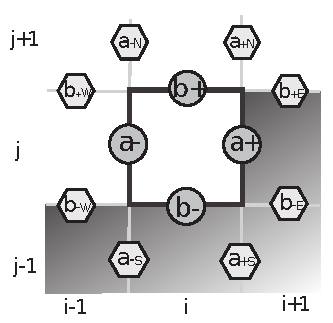
\includegraphics[height=80mm, width=8cm]{f07.pdf}
\caption{\emph{SSA stencil}}
\label{result3}
\end{center}
\end{figure}

% \begin{figure}[p!]
% \begin{center}
% \includegraphics[width=0.32\textwidth]{../plots/CF_BC_interpretation.eps}
% \caption{\emph{The calving front boundary condition is applied to determine the velocity gradients at the calving front}}
% \label{scheme}
% \end{center}
% \end{figure}

% \begin{figure}[p!]
% \begin{center}
% \includegraphics[width=0.32\textwidth]{../plots/CF_BC_coefficients.eps}
% \caption{\emph{Coefficients which are necessary to discretize the SSA equations \eqref{SSA_I} and eqref{SSA_II}. These coefficients equal zero when belonging to a calving front boundary condition and one otherwise.}}
% \label{scheme}
% \end{center}
% \end{figure}
\noindent The calving front boundary condition determines the behaviour of the velocity gradients at the calving front. To understand the implementation of the calving front boundary condition consider the SSA-equations:

\begin{align}
\frac{\partial}{\partial x}\left[ 2\bar\nu H\left( 2\frac{\partial u}{\partial x} + \frac{\partial v}{\partial y} \right)\right] + \frac{\partial }{\partial y}\left[\bar\nu H\left(\frac{\partial u}{\partial y}+\frac{\partial v}{\partial x}  \right) \right] &= \rho gH \frac{\partial h}{\partial x} \label{SSA1} \\
\frac{\partial}{\partial x}\left[ \bar\nu H\left( \frac{\partial u}{\partial y} + \frac{\partial v}{\partial x} \right)\right] + \frac{\partial }{\partial y}\left[2\bar\nu H\left(\frac{\partial u}{\partial x}+2\frac{\partial v}{\partial y}  \right) \right] &= \rho gH \frac{\partial h}{\partial y} \label{SSA2}
\end{align}
\noindent In the first step of discretization the outer derivatives yield:
\begin{align}
\frac{2}{\Delta x}N|_{i+\frac{1}{2}}^j\left( 2\frac{\partial u}{\partial x} + \frac{\partial v}{\partial y} \right)_{i+\frac{1}{2}}^j
- \frac{2}{\Delta x}N|_{i-\frac{1}{2}}^j\left( 2\frac{\partial u}{\partial x} + \frac{\partial v}{\partial y} \right)_{i-\frac{1}{2}}^j \nonumber \\
+ \frac{1}{\Delta y}N|_i^{j+\frac{1}{2}}\left(\frac{\partial u}{\partial y}+\frac{\partial v}{\partial x}\right)_i^{j+\frac{1}{2}} 
- \frac{1}{\Delta y}N|_i^{j-\frac{1}{2}}\left(\frac{\partial u}{\partial y}+\frac{\partial v}{\partial x}\right)_i^{j-\frac{1}{2}} 
&= \rho gH \frac{\partial h}{\partial x} \label{SSA1_dis1} 
\end{align}
If one or more of the nearest neighbors of the shelf box under consideration $[i,j]$ is an imfrac box or icefree ocean, the boundary between these two boxes will be a calving front and evaluating the boundary condition at these points allows to substitute the whole block which is calculated at this point:
\begin{itemize} 
\item calving front at $[i+\frac{1}{2},j]$: $\hat{n}=(1,0)$: 
\begin{align}
N|_{i+\frac{1}{2}}^j\left(2\frac{\partial u}{\partial x} + \frac{\partial v}{\partial y} \right)_{i+\frac{1}{2}}^j &= \tau_{ocean} \nonumber \\
N|_{i+\frac{1}{2}}^j\left(\frac{\partial u}{\partial y} + \frac{\partial v}{\partial x} \right)_{i+\frac{1}{2}}^j &= 0
\end{align}
\item calving front at $[i-\frac{1}{2},j]$: $\hat{n}=(-1,0)$: 
\begin{align}
N|_{i-\frac{1}{2}}^j\left(2\frac{\partial u}{\partial x} + \frac{\partial v}{\partial y} \right)_{i-\frac{1}{2}}^j &= \tau_{ocean} \nonumber \\
N|_{i-\frac{1}{2}}^j\left(\frac{\partial u}{\partial y} + \frac{\partial v}{\partial x} \right)_{i-\frac{1}{2}}^j &= 0
\end{align}
\item calving front at $[i,j+\frac{1}{2}]$: $\hat{n}=(0,1)$: 
\begin{align}
N|_{i}^{j+\frac{1}{2}}\left(\frac{\partial u}{\partial y} + \frac{\partial v}{\partial x} \right)_{i}^{j+\frac{1}{2}} &= 0 \nonumber \\
N|_{i}^{j+\frac{1}{2}}\left(\frac{\partial u}{\partial x} + 2\frac{\partial v}{\partial y} \right)_{i}^{j+\frac{1}{2}} &= \tau_{ocean}
\end{align}
\item calving front at $[i,j-\frac{1}{2}]$: $\hat{n}=(0,-1)$: 
\begin{align}
N|_{i}^{j-\frac{1}{2}}\left(\frac{\partial u}{\partial y} + \frac{\partial v}{\partial x} \right)_{i}^{j-\frac{1}{2}} &= 0 \nonumber \\
N|_{i}^{j-\frac{1}{2}}\left(\frac{\partial u}{\partial x} + 2\frac{\partial v}{\partial y} \right)_{i}^{j-\frac{1}{2}} &= \tau_{ocean}
\end{align}
\end{itemize}
By rewriting equation \eqref{SSA2} these boundary conditions can be taken into account:
\begin{align}
&\qquad a_+\frac{2}{\Delta x}N|_{i+\frac{1}{2}}^j\left( 2\frac{\partial u}{\partial x} + \frac{\partial v}{\partial y} \right)_{i+\frac{1}{2}}^j
- a_-\frac{2}{\Delta x}N|_{i-\frac{1}{2}}^j\left( 2\frac{\partial u}{\partial x} + \frac{\partial v}{\partial y} \right)_{i-\frac{1}{2}}^j \nonumber \\
+ &\qquad b_+\frac{1}{\Delta y}N|_i^{j+\frac{1}{2}}\left(\frac{\partial u}{\partial y}+\frac{\partial v}{\partial x}\right)_i^{j+\frac{1}{2}} 
- b_-\frac{1}{\Delta y}N|_i^{j-\frac{1}{2}}\left(\frac{\partial u}{\partial y}+\frac{\partial v}{\partial x}\right)_i^{j-\frac{1}{2}} \nonumber \\
= &\qquad \rho gH \frac{\partial h}{\partial x} + (a_+ - a_-)\frac{2}{\Delta x}\tau_{ocean} \label{SSA1_dis2}
\end{align}
$a_\pm$ and $b_\pm$ equal zero if the boundary is a calving front and one otherwise. Next, the calculation of the velocity gradients is further specified by rewriting these in a way that allows to calculate the derivatives as differential quotient between two neighboring points:
\begin{align}
&\qquad a_+\frac{4}{\Delta x}N|_{i+\frac{1}{2}}^j\left[ a_+\frac{\partial u}{\partial x}_{i+\frac{1}{2}}^j + \frac{1}{8}\left( b_{+E}\frac{\partial v}{\partial y}_{i+1}^{j+\frac{1}{2}}+b_{-E}\frac{\partial v}{\partial y}_{i+1}^{j-\frac{1}{2}}+b_+\frac{\partial v}{\partial y}_{i}^{j+\frac{1}{2}}+b_-\frac{\partial v}{\partial y}_{i}^{j-\frac{1}{2}}  \right) \right] \nonumber \\
- &\qquad a_-\frac{4}{\Delta x}N|_{i-\frac{1}{2}}^j\left[ a_-\frac{\partial u}{\partial x}_{i-\frac{1}{2}}^j + \frac{1}{8}\left( b_+\frac{\partial v}{\partial y}_{i}^{j+\frac{1}{2}} + b_-\frac{\partial v}{\partial y}_{i}^{j-\frac{1}{2}} + b_{+W}\frac{\partial v}{\partial y}_{i-1}^{j+\frac{1}{2}} + b_{-W}\frac{\partial v}{\partial y}_{i-1}^{j-\frac{1}{2}} \right) \right] \nonumber \\
+ &\qquad b_+\frac{1}{\Delta y}N|_i^{j+\frac{1}{2}}\left[ b_+\frac{\partial u}{\partial y}_i^{j+\frac{1}{2}}+\frac{1}{4}\left( a_{+N}\frac{\partial v}{\partial x}_{i+\frac{1}{2}}^{j+1} + a_+\frac{\partial v}{\partial x}_{i+\frac{1}{2}}^{j} + a_{-N}\frac{\partial v}{\partial x}_{i-\frac{1}{2}}^{j+1} + a_-\frac{\partial v}{\partial x}_{i-\frac{1}{2}}^{j} \right) \right] \nonumber \\
- &\qquad b_-\frac{1}{\Delta y} N|_i^{j-\frac{1}{2}} \left[ b_-\frac{\partial u}{\partial y}_i^{j-\frac{1}{2}}+\frac{1}{4}\left( a_+\frac{\partial v}{\partial x}_{i+\frac{1}{2}}^{j} + a_{+S}\frac{\partial v}{\partial x}_{i+\frac{1}{2}}^{j-1} + a_-\frac{\partial v}{\partial x}_{i-\frac{1}{2}}^{j} + a_{-S}\frac{\partial v}{\partial x}_{i-\frac{1}{2}}^{j-1} \right) \right] \nonumber \\
%%
= &\qquad \rho gH \frac{\partial h}{\partial x} + (a_+ - a_-)\frac{2}{\Delta x}\tau_{ocean} \label{SSA1_dis3}
\end{align}
Again, the coefficents $a_{\pm N,S}$, $b_{\pm E,W}$ etc. are determined by the nature of the boundary between the two points used to calculate the differential quotient: zero if it is a calving front boundary and one if it is an ice-ice boundary. Thus an ice-inward scheme is used to calculate velocity gradients,  justified by assuming that the only influence of the ocean on the shelf is by exerting the extra pressure introduced on the right hand side of equation \eqref{SSA1_dis3}. The second SSA-equation \eqref{SSA2} is discretized accordingly.



\begin{thebibliography}{2}
\bibitem{Bueler2008a} Bueler and Brown (2008), The shallow shelf approximation as a "sliding law" in a thermomechanically coupled ice sheet model, \emph{submitted} 
\bibitem{Bueler2008b} Bueler, Brown, Shemonski, Khroulev (2008), PISM user's manual: A parallel ice heet model, \emph{http://www.pism-docs.org/manual-dev.pdf} 
\bibitem{MacAyeal96} MacAyeal et al. (1996), An ice-shelf model test based on the Ross Ice Shelf,
Antarctica, Ann. Glaciol., 23
\bibitem{Morland87} Morland, L.W. (1987), Unconfined Ice-Shelf flow,
In van der Veen and Oerlemans, eds. Dynamics of the West Antarctic Ice Sheet, 99-116 
\bibitem{Weis01} Weis (2001), Theory and Finite Element Analysis of Shallow Ice Shelves
\end{thebibliography}

\end{document}